\section{Blockchain technology}
\label{sec:blockchain}

"Do you need a blockchain?" was a breaking paper describing that most use cases do not need blockchain technology \cite{Wust2018}.
At a surface level, blockchain shares structural similarities with distributed NoSQL databases such as MongoDB: both store data across multiple nodes and support replication \cite{Chowdhury2018}.
However, the fundamental difference lies in the trust model. A NoSQL database operates under the assumption that all participating nodes are honest and controlled by a single administrative entity. Blockchain, by contrast, is designed for adversarial environments where participants may act maliciously, and it relies on consensus algorithms to ensure that state transitions are valid without requiring trust in any single party \cite{Du2017}.
The key properties that distinguish blockchain from traditional distributed databases are \cite{Zheng2017}:

\begin{enumerate}
    \item \textbf{Immutability} -- once data is committed to the chain, it cannot be altered or deleted without invalidating subsequent blocks, providing a tamper-evident audit trail.
    \item \textbf{Trust minimization} -- participants can verify the correctness of state transitions independently through cryptographic proofs and consensus, eliminating the need to trust a central authority.
    \item \textbf{Accessibility} -- depending on the network type (permissionless, permissioned, or semi-permissioned), participants can read from and write to the ledger according to the network's access policy.
    \item \textbf{Decentralization} -- the ledger is replicated across geographically distributed nodes, eliminating single points of failure and censorship.
\end{enumerate}

When we want to add or modify the data from the blockchain, we need to create new updates to the chain called a transaction.
These updates are done in batches, so-called blocks, and each block consists of many transactions that can modify the state of the blockchain.
Each blockchain stores different data in the block for the correct functioning. These data depends on the selected consensus algorithm or the implementation of the blockchain.
In general, the data structure of the blockchain is the following:

\begin{itemize}
  \item height - the number of the block,
  \item timestamp - the time when the miner created the block,
  \item hash - the hash of the Merkle tree of all transactions in the block,
  \item parent hash - the hash of the previous block,
  \item transactions - the list of transactions in the block,
  \item creator - the creator of the block.
\end{itemize}


However, to properly update the state, we need a genuine algorithm that can decide about the participant of the network that can validate the block validity.
This algorithm is known as the consensus algorithm. Formally, a consensus protocol must satisfy two fundamental properties: \textit{safety}, ensuring that all honest nodes agree on the same state and no conflicting transactions are finalized, and \textit{liveness}, guaranteeing that valid transactions are eventually included in the ledger. In the presence of malicious actors, these guarantees are studied under the framework of Byzantine fault tolerance (BFT), where the system can tolerate up to a threshold of faulty or adversarial nodes \cite{Du2017}.

In the area of blockchain, there are many types of consensus algorithms. The most common are \cite{Bach2018}:

\begin{itemize}
  \item[ ] Proof-of-Work (PoW) - The idea behind the Proof-of-Work is that to make a valid block; we need to use extensive computational resources to find a correct value in the cryptographical puzzle.
  \item[ ] Proof-of-Stake (PoS) - Uses the participants' stake to decide the block's validity.
  \item[ ] Nominated Proof-of-Stake (NPS) - a Proof-of-Stake with the possibility of other participants nominating their stake to the block validator
  Therefore, the block reward is split between the validator and other nominators by the ratio of their stake. The NPOS is used in the Polkadot and their parachains.
\end{itemize}

Now we have immutable finalized data, finalized trustlessly over the network using a consensus algorithm. How can we access the data?
That is a crucial question. The answer is not very simple. By the nature of the blockchain, we know three types of access \cite{Zheng2017}:

\begin{itemize}
  \item permissionless,
  \item permissioned,
  \item semi-permissioned.
\end{itemize}

Decentralized means that the blockchain is distributed across the network. As we can see in Figure \ref{fig:decentralized}, blockchain nodes hold the same information state instead of having one single source of truth.
Therefore, having this ability to read the data from the blockchain, we can access the state from any node in the network.

\begin{figure}[!ht]
  \centering
  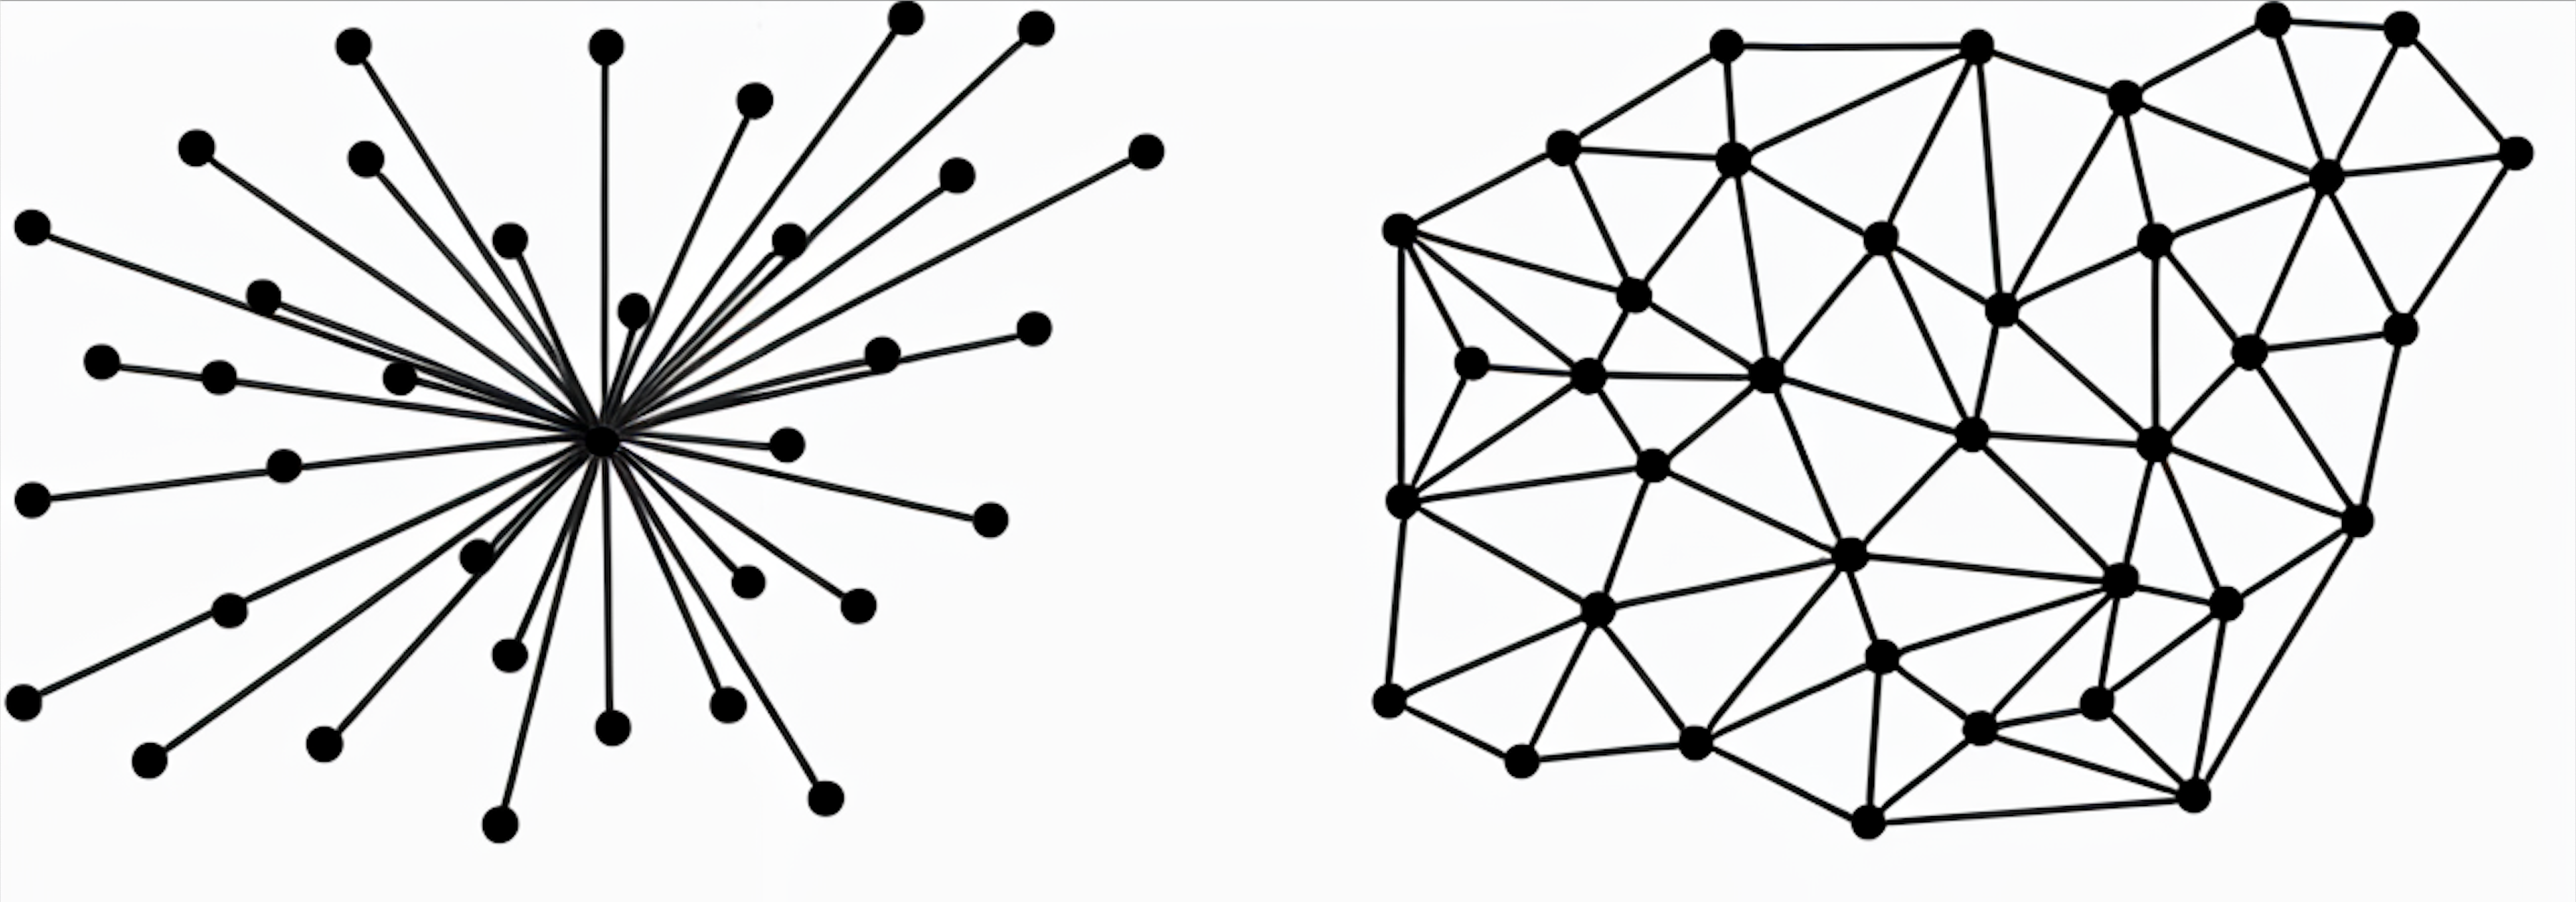
\includegraphics[width=\columnwidth]{images/distributed.png}
  \caption{Graphical representation of centralized and distributed network \cite{baran1964distributed}}
  \label{fig:decentralized}
\end{figure}


\subsection{Smart contracts}

A smart contract is a deterministic program deployed on a blockchain that automatically enforces predefined rules when triggered by a transaction \cite{szabo1997contracts}. Unlike traditional legal contracts, which require trusted intermediaries for enforcement, smart contracts derive their guarantees from the underlying consensus mechanism: once deployed, their execution is verified by all participating nodes, making the outcome tamper-proof and publicly auditable \cite{DeFilippi2018}.
How do smart contracts work? The smart contract is a program running on blockchain written in Turing-complete\footnote{In the context of EVM, Bitcoin Script is Turing-incomplete} programming language \cite{szabo1997contracts}.
To deploy a smart contract, we need to create a smart contract code, compile it into the binary code and then send it to the blockchain as a transaction.
Once the contract is deployed, it gets a unique address that is used to access the contract and the storage where we can store the data.
By default, the smart contract code is immutable. However, a proxy contract can be used to change the code of the contract \cite{wood2014ethereum}.

The first blockchain that brought the concept of smart contracts is Ethereum. In high overview, the Ethereum blockchain has an Ethereum Virtual Machine (EVM) that is used to run smart contracts.
Thanks to the Turing completeness of the EVM, when we want to write a smart contract can use one of the high-level programming languages like Solidity or Vyper \cite{antonopoulos2018mastering}.
However, the EVM does not directly execute code from the smart contract language. Instead, the code is compiled into the EVM bytecode.
To make the computation sustainable, when we want to make a transaction, we need to pay a fee defined by the gas \cite{Leonardos2021, Roughgarden2020}. Using gas serves as the fee for miners to include the transaction into block. Additionally a tip can be included for faster transaction processing.
As every code byte requires a fee to be executed, we are trying to make the smart contract as efficient as possible. How to do that?
To write compelling and safe smart contracts, communities created
open-source libraries like OpenZeppelin\footnote{https://github.com/OpenZeppelin/openzeppelin-contracts} or Solmate\footnote{https://github.com/transmissions11/solmate} that can help us to complete our goal.

% Something about open-zeppelin and smart contract security?

Nevertheless, the main question is how smart contracts can bring value.
Since smart contracts can call other smart contracts, we need to bring a set of APIs or standardizations that can be used to access and modify the data.
One of the most fundamental standards in the blockchain ecosystem is tokens. We can imagine a token as a digital asset representing something with a monetary value (e.g. being used to pay for services).
Or it can be a unique, non-fungible item that can represent either a physical, real-world object,
therefore a token is a digital twin or a digital asset that can be later reused for various use cases, such as identity pass or the object in the metaverse.
The most common reference standards across various blockchain ecosystems are Ethereum Improvement Proposals or EIPs.

The EIPs are a set of proposals that are designed to bring value or improve the existing standards in the network.
The four main EIPs for fungible and non-fungible tokens are ERC-20, ERC-721, ERC-777, and ERC-1155.

We need to choose the right token type depending on the use case. To create a fungible, use ERC-20.
What are the fungible tokens in general? We can say that they are tokens that can be interchangeable \cite{vogelsteller2015erc}.
As an example, one USD bill has the same monetary value as another USD bill. In the space of cryptocurrencies,
many projects make their tokens to cover different use cases. In the case of the blockchain-based car-sharing platform \cite{valastin2019} we can create a fungible token that would be distributed as a reward for using the car-sharing service.
This token can be used to get a discount for the next ride. In summary, ERC-20 tokens are a simple tool to create and share fungible value.
However, its simple architecture brings some caveats that we need to consider. That is the reason ERC-777 was created.
The best feature of the ERC-777 standard is the so-called receive hooks \cite{Dafflon2017}.
Using ERC-777 instead of ERC-20 prevents us or other smart contracts from accidentally sending other tokens to the contract and bricking them \cite{EIP777}.

Nevertheless, what if we want to create a non-fungible token? ERC-721 is the answer.
ERC-721 is a standard that allows us to create tokens that are not interchangeable \cite{entrikennon}.
Often we can use ERC-721 to create a token that represents a tokenized physical object.
In the previously mentioned car-sharing platform \cite{valastin2019}, we use non-fungible tokens to represent a car.
Moreover, thanks to the composable architecture, we can also represent keys for the car in the form of NFT owned by the car itself.
In 2021 NFT got into the mainstream. Many people created their own collectible ERC-721 smart contracts that could be later sold on the blockchain-based marketplace.
Nevertheless, how to distinguish between the two unique tokens? Many tokens hold additional metadata in the form of JSON \cite{entrikennon, Morgan2018} using predefined schema.

Where is the metadata stored? This question is architecturally significant because the choice of storage directly affects key value dimensions of digital assets: availability (whether the metadata remains accessible), durability (whether it persists over time), and mutability (whether it can be updated). Since on-chain storage is prohibitively expensive for large data, the ecosystem has developed several decentralized storage solutions \cite{Benet2014, Wilkinson2014, Williams2019}.
Table \ref{table:storages} compares these alternatives along dimensions relevant to our value framework \cite{Daniel2022}.

\begin{table}[ht]
  \centering
  \caption{Comparison of token types to token functions}
  \begin{tabular}{ |p{2cm}|p{3.5cm}|p{3.5cm}|p{3.5cm}| }
  \hline
          & IPFS & StorJ & Arweave                                 \\
  \hline
  Availability  & Temporary & While we pay & Permanent     \\
  \hline
  Mutability  &  yes via IPNS & yes & no     \\
  \hline
  Goal &  fast data distribution & decentralized cloud storage & permanent data storage     \\
  \hline
  Feature & Easy-to-use    & Private storage   & Smart Contracts     \\
  \hline
  Price per 1GB\footnote{(\$/month)} & 0.15\footnote{https://pinata.cloud/pricing}    & 0.004\footnote{https://www.storj.io/pricing}  & 5-7.5 (forever)\footnote{https://ardrive.io/pricing/}     \\
  \hline
  \end{tabular}
  \label{table:storages}
  \end{table}

What if we wanted to create both fungible and non-fungible tokens within one contract? Currently, ERC-20 or ERC-721 requires us to create a new smart contract for each new collection.
ERC-1155 addresses this by allowing a single smart contract to hold multiple token collections, both fungible and non-fungible, within one deployment.
This is particularly beneficial for games that need a blockchain to store fungible game assets, such as gold or silver, alongside unique items with traits like armour.
Batch operations in ERC-1155 can reduce transaction fees by up to 80\% compared to equivalent operations across separate ERC-20 and ERC-721 contracts \cite{EIP1155}.

However, what if we want to represent more complex assets, such as tokenized houses or a gaming character, using an inventory of items accumulated over time? It is undoubtedly possible with current ERC-721 and  ERC-1155 standards, but it will introduce complexity to the implementation and decrease composability.

Proposed ERC-6551 addresses this gap by creating a so-called smart contract wallet for each ERC-721 item in the collection. Thanks to this token-bound account principle, a token can own other fungible and non-fungible tokens, thereby making a composable entity out of a non-fungible token \cite{EIP6551}. Nevertheless, ERC-6551 is not the first attempt to create composable non-fungible tokens. Valastin et al. created a blockchain-based car-sharing platform using ERC-998 to represent the relationship between a car and its key. The problem with this approach is that this logic has to be implemented inside a smart contract \cite{valastin2019, EIP998}. On the other hand, any ERC-721 token could be upgraded to a token-bound account via ERC-6551 without any modifications.

Along with composability, ERC-6551 provides a perfect substrate for creating AI agents, even though there is no unified standard for obtaining information about particular AI agents and their capabilities. The novel standard ERC-8004 fixes this by extending ERC-721 metadata with additional fields regarding agent capabilities, goals, and relevant information. Why is this needed? To create an analogy with traditional NFTs that contain attributes, agents expose endpoints for services. Additionally, ERC-8004 exposes smart contract calls to attach on-chain ratings to the agent\cite{EIP8004}.

% As we look at Table \ref{table:tokencomparison}

% \begin{table}[ht]
%   \centering
%   \caption{Comparison of token types to token functions}
%   \begin{tabular}{ |c|c|c|c|c| }
%   \hline
%           & ERC-20 & ERC-721 & ERC-1155                                 \\
%   \hline
%   Batch transfer & Yes    & No      & Yes                                       \\
%   Hold metadata & No    & Yes     & Yes                                          \\
%   Use as collateral & Yes    & Yes     & Yes                                       \\
%   \hline
%   \end{tabular}
%   \label{table:tokencomparison}
%   \end{table}

What do smart contracts in Polkadot ecosystems look like?

Similarly to Ethereum, Polkadot has its own virtual machine called PolkaVM. It is a RISC-V-based virtual machine that is able to run Solidy smart contracts. 
In contrast to Ethereum, multiple smart conctract laguages can compile to RISC-V code and therefore offers higher flexibility compared to EVM.
However, the ecosystem around Polkadot smart contracts is still evolving. What makes the ecosystem unique is the ability to create custom, extendable logic for the blockchain, which we will cover in the subsection \ref{subsec:pallets}.

\subsection{Substrate and runtime modules} \label{subsec:pallets}

When we want to build our blockchain tailored to our needs, we have three options:

\begin{itemize}
  \item Start from scratch,
  \item For the existing blockchain, we can use the existing code and add new functionality.
  \item Use an abstract framework to build our blockchain.
\end{itemize}

In the first case, we need to write our code, consensus and run many tests. However, this is an excellent approach to conducting research with a high possibility of inventing something new.
It usually never reaches the point of success or practical application.
The second case was the most common approach to building a blockchain. Most of the time, projects forked Bitcoin or Ethereum network, tweaked the functionality and modified some underlying code.
However, it was a usual way that it did not provide the flexibility to update code from the upstream or did not guarantee that these blockchains would be interoperable.

The third case leverages modular blockchain frameworks that abstract networking, consensus, and storage layers, allowing developers to focus on application-specific logic. Analogous to how web frameworks like NuxtJS abstract server configuration and routing, blockchain frameworks provide pre-built, audited implementations of consensus algorithms, peer-to-peer networking, block finalization, and account management.
The practical advantage is twofold: developers avoid reimplementing security-critical infrastructure, and the resulting chains remain interoperable with other networks built on the same framework \footnote{https://docs.substrate.io/fundamentals/why-substrate}. For this thesis, we adopt the framework-based approach because our contributions lie in the application layer (value assessment and agentic execution), not in consensus design.


The focus of this thesis is Substrate, a modular blockchain framework developed by Parity Technologies. It is important to distinguish Substrate from Polkadot: Substrate is the generic framework for building blockchains, while Polkadot is a specific multi-chain network built using Substrate that provides shared security and cross-chain interoperability for its connected parachains \cite{Wood2017}. Any blockchain built with Substrate can operate independently or opt into the Polkadot network.
From the node perspective, a Substrate-based blockchain has two main components\footnote{https://docs.substrate.io/fundamentals/architecture}:

\begin{itemize}
  \item Node - the part of the code that is running on the network,
  \item Runtime - the part of the code that is running on the node.
\end{itemize}

As shown in Figure \ref{fig:substrate-arch}, the node part has a couple of responsibilities, such as communication between nodes, allowing clients to fetch data via Remote Procedure Calls (RPC) and storing information of the blockchain.
The runtime part is the part of the code running on the node. It is responsible for correcting the storage mutation and executing the business logic.
% Some more sentences + picture

\begin{figure}[!h]
  \centering
  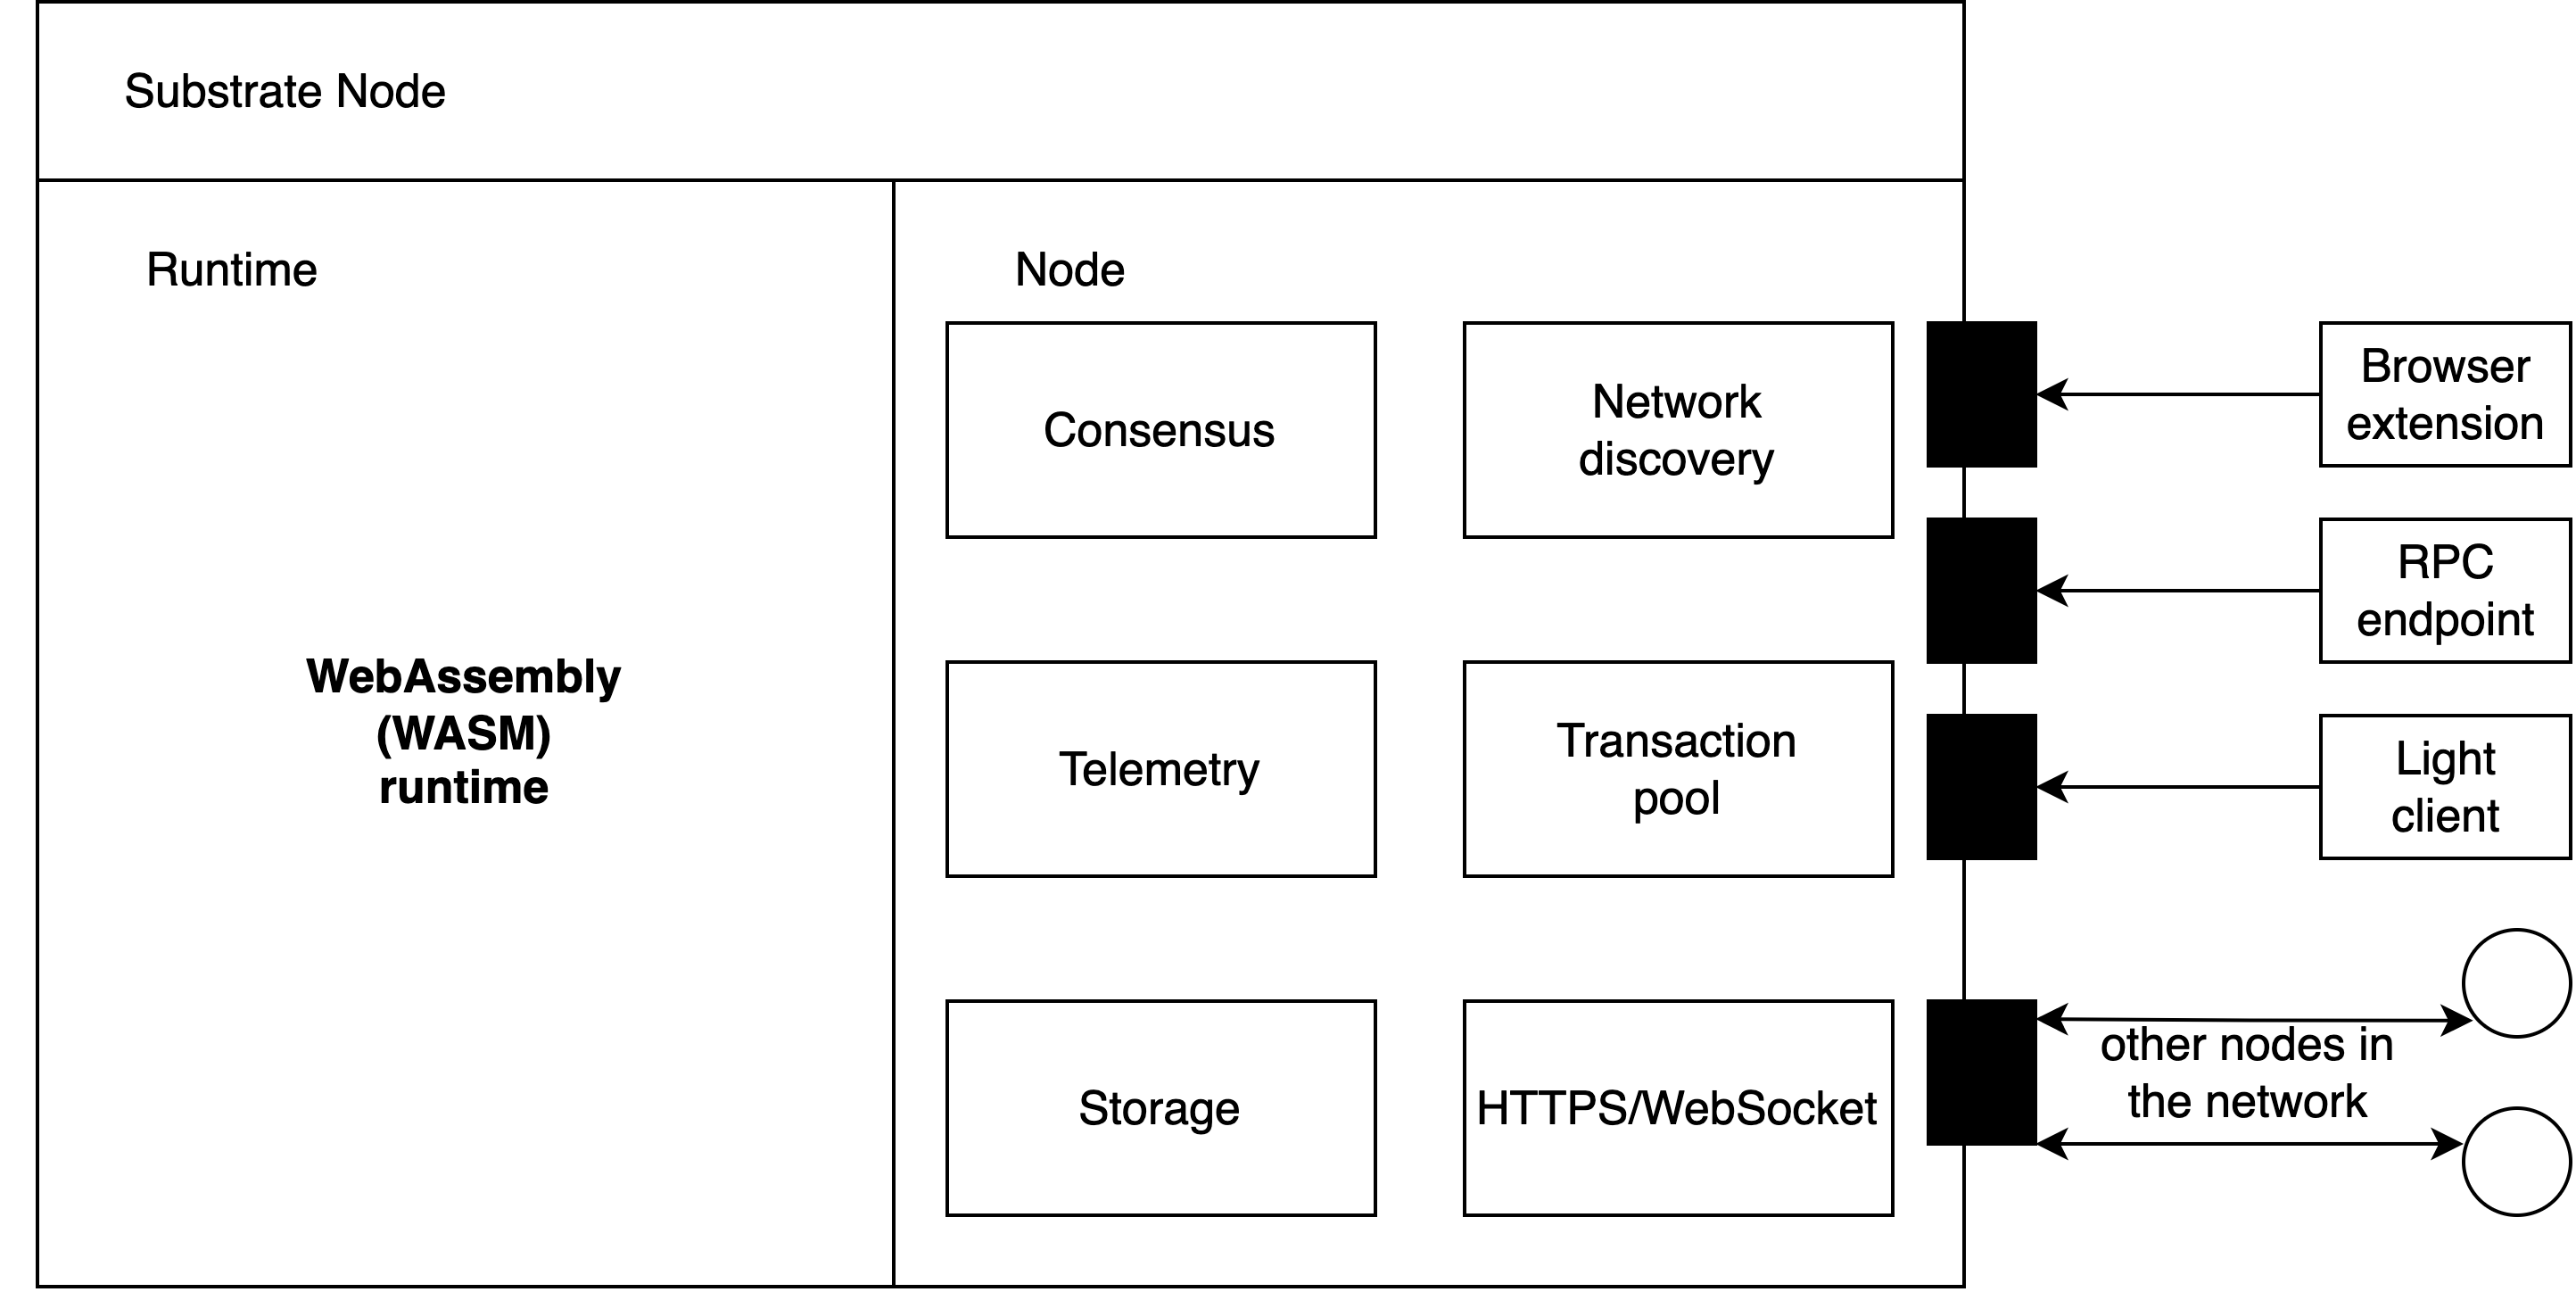
\includegraphics[width=\columnwidth]{images/substrate-architecture.png}
  \caption{Substrate architecture \cite{Johnson2019}}
  \label{fig:substrate-arch}
\end{figure}

Thanks to the Substrate framework's modular nature, we can create custom logic for our blockchain.
As we discussed, the node's runtime is responsible for executing all the business logic \cite{Tabrizi2018}.
The core of the modular blockchain has a toolset for tweaking the runtime. This tooling is called Framework for Runtime Aggregation of Modularized Entities (FRAME).
FRAME consists of tools and modules that can be used to build a custom runtime.
This custom blockchain logic is called the runtime module or pallet in general. If we look at Figure \ref{fig:frame-runtime}, we see that the, by default, Substrate-based blockchain can consist of many pallets.
The core set of pallets (around 40 of them) contains critical pallets like accounts, staking, governance, and many more.

\begin{figure}[!h]
    \centering
    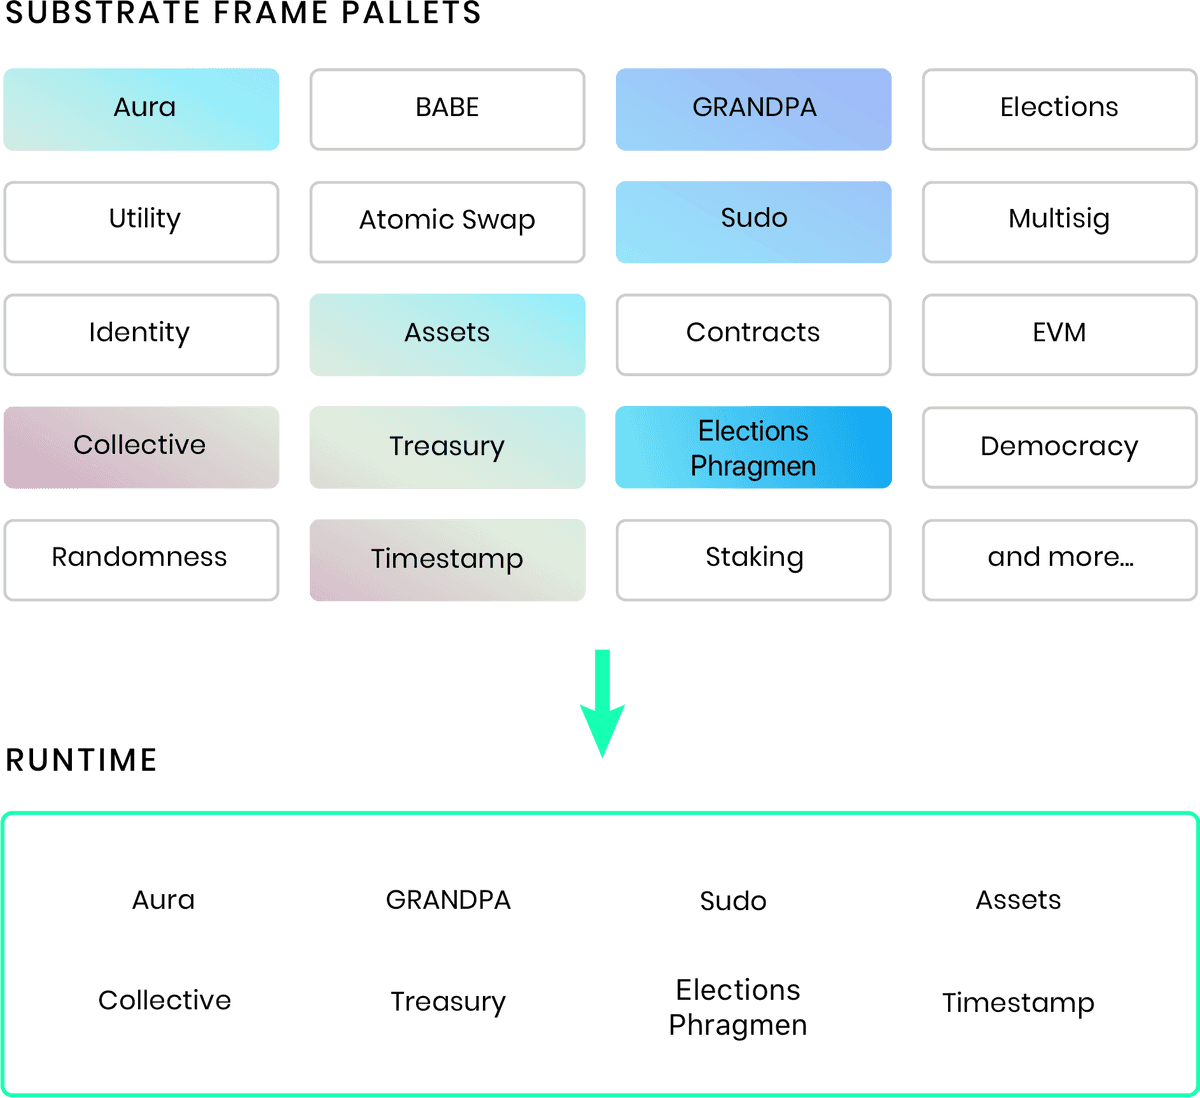
\includegraphics[width=\columnwidth]{images/frame-runtime.png}
    \caption{Substrate runtime modules}
    \label{fig:frame-runtime}
\end{figure}

A pallet is a self-contained Rust module that encapsulates a specific piece of blockchain logic (e.g., token balances, staking, governance) along with its own storage, callable functions, and events. Pallets interact through well-defined trait interfaces, enabling composition without tight coupling. For example, the staking pallet in Polkadot delegates balance operations to the balances pallet via a shared \texttt{Currency} trait: it instructs the balances pallet to lock a portion of tokens for staking, while remaining agnostic to how balances are internally managed \cite{Burdges2020, Abbas2022}. This modularity is central to our work, as we implement our contributions (such as the NFTAA primitive) as custom pallets that compose with existing infrastructure.

We briefly illustrate the pallet structure below, as our NFTAA implementation (Chapter~\ref{sec:design}) follows the same pattern. Each pallet consists of four main parts
\begin{enumerate}
    \item Runtime Storage,
    \item Extrinsic,
    \item Runtime Events,
    \item Hooks.
\end{enumerate}

Same as in the smart contracts, storage can hold variables which are either primitive type, map or double map. As shown in Listing \ref{lst:storage} below, we have a variable named \verb|Something| is a type of unsigned 32-bit integer. To fetch the current value from the chain, Substrate offers a Rust-based macro \verb|#[pallet::getter()]|. Pallet macros help us to hide a ton of complex and boilerplate code from the pallet, so the result is that Rust code is easier to read for smart contract programmers.

\begin{lstlisting}[caption={Defining storage variable in Substrate runtime pallet},label={lst:storage}]
  #[pallet::storage]
  #[pallet::getter(fn something)]
  pub type Something<T> = StorageValue<_, u32>;
\end{lstlisting}

The second part of the pallets is extrinsic. These functions are called when we make a transaction to the blockchain and are allowed to change the state of the storage.
As shown in Listing \ref{lst:extrinsic} function \verb|do_something| is changing the value of variable \verb|Something| defined in the storage show in Listing \ref{lst:storage}. At the end of the function, we dispatch an event that tells us the value we stored and our address.

\begin{lstlisting}[caption={Defining extrinsic in Substrate runtime pallet},label={lst:extrinsic}]
  pub fn do_something(origin: OriginFor<T>, something: u32) -> DispatchResult {
    let who = ensure_signed(origin)?;
    <Something<T>>::put(something);
    Self::deposit_event(Event::SomethingStored(something, who));
    Ok(())
  }
\end{lstlisting}

The last part of the pallets is events. In the same manner, as in smart contracts, we need to emit some status if the call was successful or not. This is done by emitting an enum from \verb|Event| as shown in Listing \ref{lst:events}.


\begin{lstlisting}[caption={Defining events in Substrate runtime pallet},label={lst:events}]
	#[pallet::event]
	#[pallet::generate_deposit(pub(super) fn deposit_event)]
	pub enum Event<T: Config> {
		SomethingStored(u32, T::AccountId),
	}
\end{lstlisting}

% https://docs.substrate.io/v3/runtime/frame/
% https://github.com/vikiival/salt-mine

Thanks for the portability and flexibility EVM compatibility for PolkaVM is implemented as a pallet called revive.

\subsection{Final thoughts on decentralized ledger technology}

Blockchain opens a new world of possibilities as a decentralized ledger technology.
Using a piece of code that can be executed without needing a trusted third party, we can build new exciting use cases that can enhance the Internet of Value.
The emerging sector of decentralized finance allows us to use our money non-stop and without restrictions\cite{Jensen2021, Schar2021, Zetzsche2020}. Moreover, the technology is open to the public and can be used by anyone. So, we can compose tokens into a new product
that can create additional profit. Unique assets can be tokenized and traded via the Internet, using minimal transaction costs. Companies such as OpenZeppelin are building effective and safe smart contracts.
Although there are many blockchain technologies, the most popular one is Ethereum. Emerging Substrate framework is a technology that can help us to build a fast, effective and modular blockchain.
The next Chapter \ref{sec:analysis} will go through the importance of IoV and the use cases that can be built with it.
